In this section we introduce and define some of the concepts that were necessary for this project.

\subsection{Boundary layer structure}
The planetary boundary layer or atmospheric boundary layer (ABL) is defined as the part of the troposphere that is in contact with the surface and that is directly influenced by surface forcings, such as friction, evaporation, heat transfer, emission of contaminants and by the soil~\citep{stull2012introduction}. The thickness or height of the ABL varies throughout the day and depends on the location. Mainly the height varies by the incidence of solar radiation on the surface, which makes the air parcels in contact with the surface acquire more flotation, generating convection.

\begin{figure}[ht!]
	\vspace{-5pt}
    \centering
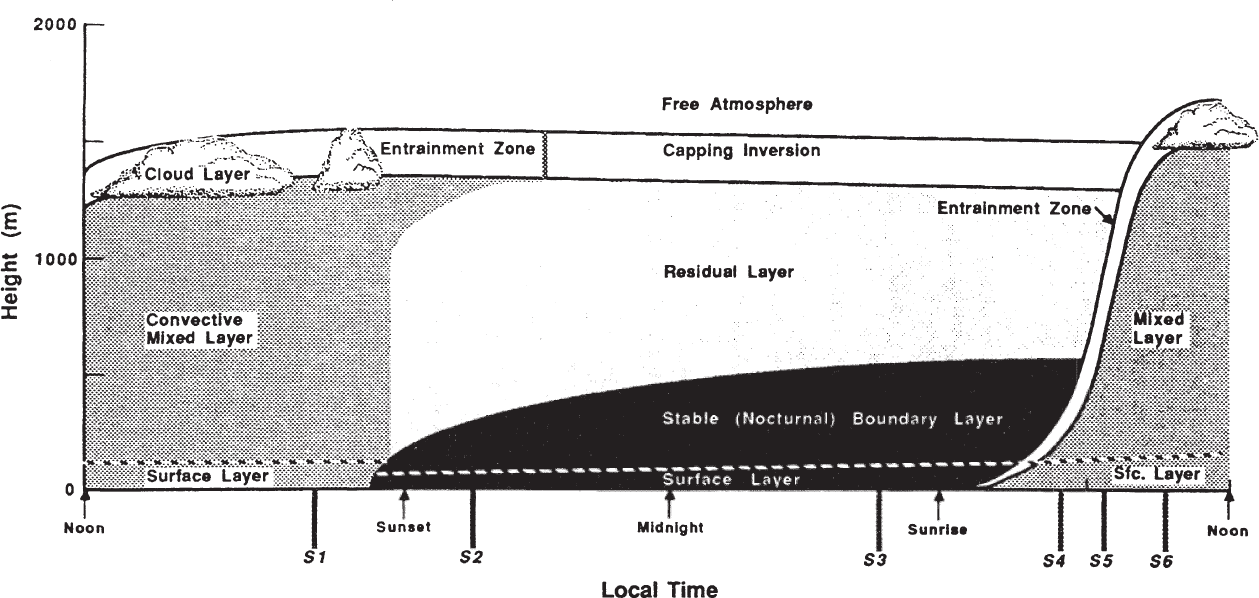
\includegraphics[width=0.9\textwidth]{fig/abl_stull.png}
    \caption{Diagram of the daily evolution of the structure of the ABL. Image based on \cite{stull2012introduction}.}
    \label{fig:ABL_structure}
  \vspace{-5pt}
\end{figure}

The figure~\ref{fig:ABL_structure} shows the structure and temporal evolution of the ABL, its components are the mixing layer, the residual layer and the stable boundary layer. Each of these has special characteristics and different physical processes that distinguish them. To understand the dynamics of the planetary boundary layer it is necessary to define each of them. However, in this study, we focus mostly on the stable nocturnal boundary layer because in the presence of this layer katabatic winds form~\citep{poulos2008observational, stull2012introduction}.

\subsubsection{Stable boundary layer}
The stable nocturnal boundary layer is formed during the night when the sunlight stops reaching the ground and therefore starts cooling down. This layer is characterised by sporadic turbulence caused by wind shear and the contact with the surface, which tends to suppress turbulence. The upper limit of the stable boundary layer is located at the height where the intensity of the turbulence is a small fraction of its surface value. The air in this layer is statically stable, opposed as its daytime equivalent, the mixed layer~\citep{stull2012introduction}.

When the stable boundary layer is formed, the air that is close to the ground cools down and can form drainage winds or katabatic winds, over a slope in the topography.

\subsection{Katabatic wind} \label{sec:katabatic_winds}

The katabatic winds are local winds that are created over a descending terrain gradient when air masses flow downslope, being cooled by radiative processes near the ground. These winds are a ventilation mechanism in mountainous regions~\citep{manins1979model}. Normally, these winds are shallow, where the thickness of the jet can go up to 2-3~m, with velocities on the order of 1 to 5~m/s \citep{stull2012introduction}. 

\begin{figure}[ht!]
	\vspace{-5pt}
    \centering
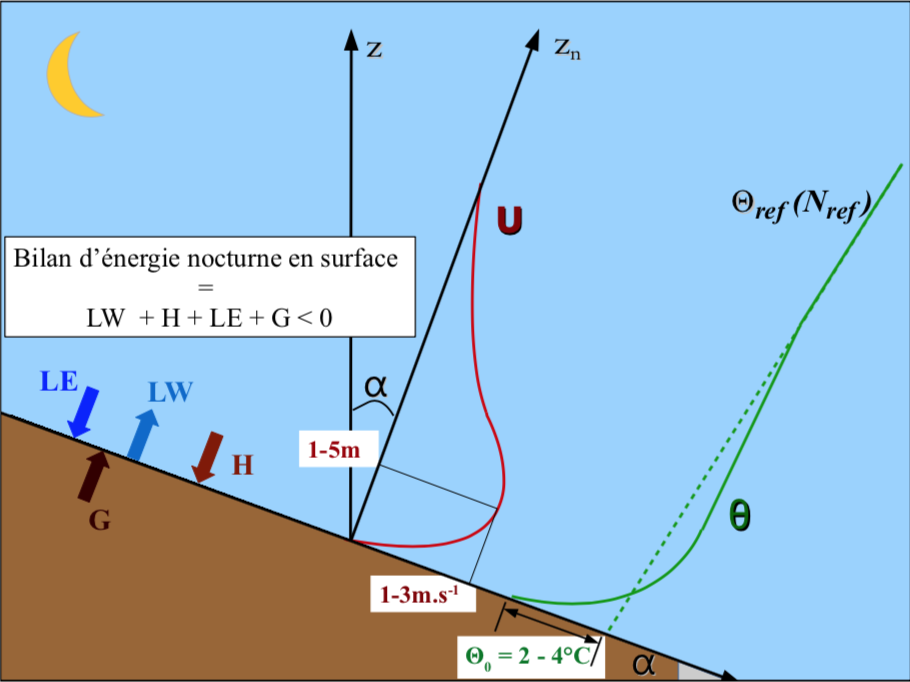
\includegraphics[width=0.6\textwidth]{fig/profiles_katabatic_wind.png}
    \caption{Characteristic wind profile (red) and potential profile (green) of the katabatic wind. Image from~\cite{claudine}.}
    \label{fig:u_profile}
  \vspace{-5pt}
\end{figure}

These winds are characterised for having a velocity profile as the one shown in the red curve in figure~\ref{fig:u_profile}, where is possible to see that the maximum speed is located near the surface. This is the theoretical velocity profile of the katabatic winds. Also in figure~\ref{fig:u_profile}, we can see in the green curve the profile for the potential temperature, where the theoretical profile shows that it grows rapidly as we go up until a point were it remains constant. This theoretical results can be useful to detect the occurrence of katabatic wind in the data sets.

An important factor to highlight about the katabatic winds is that external factors like synoptic or mesoscale winds can alter or destroy this kind of local winds~\citep{stull2012introduction}. The katabatic winds are important under conditions of slack synoptic pressure gradients~\citep{manins1979katabatic}. This factor plays an important role in the planning out the field campaign because we want to measure the katabatic jet as undisturbed as possible.

%\subsection{Governing equations}

\subsection{Turbulence Kinetic Energy (TKE)}
The TKE is defined as the kinetic energy per unit mass. This is one of the most important quantities to characterise turbulence in a flow, by giving us information about whether a region will become more turbulent, or whether turbulence will decay~\citep{stull2012introduction}.  Is defined as:

\begin{equation}
    TKE = \frac{1}{2} \big(\overline{u'^2} + \overline{v'^2} + \overline{w'^2}\big). 
    \label{eq:tke}
\end{equation}

\noindent where $TKE$ is the definition of turbulent kinetic energy (TKE). Is the sum of the variances of the wind components fluctuation. The over-line represents the average of the variable. 

\subsection{Covariance}

Recalling the classical definition of covariance between to variables, we have the relation 

\begin{equation}
    \text{covar}(A,B) = \frac{1}{N}\sum_{i=0}^{N-1} (A_i - \overline{A})(B_i - \overline{B}).
\end{equation}

\noindent Using the Reynolds averaging method in the previous expression we get:

\begin{subequations}
\begin{align}
    \text{covar}(A,B) &= \frac{1}{N}\sum_{i=0}^{N-1} a_i' b_i', \\
    &= \overline{a'b'}.
\end{align}
\end{subequations}

\noindent This is the mathematical definition of covariance. The covariance indicates the degree of common relationship between two variables. Is the principle by which we define the eddy fluxes.

\subsection{Eddy Flux}
According to \cite{stull2012introduction}, a turbulent flux or eddy flux is the transport of a physical quantity by the effect of the turbulence. In this project, we are mostly concerned with the sensible heat flux and the momentum flux. The sensible heat flux is given by the expression:

\begin{equation}
    H = \rho \ C_p \ \overline{w'\theta'},
\end{equation}

\noindent where $C_p$ is the specific heat at constant pressure and $\theta '$ is the fluctuations in potential temperature. We are interested in the vertical flux of the sensible heat, that is why we use the vertical wind fluctuation $w'$.

The momentum flux is given by the expression

\begin{equation}
    F = \rho \ \overline{u'w'}, 
\end{equation}

\noindent where $\rho$ is the density of air, and $u'$ and $w'$ are the fluctuations of velocity in the x-coordinate and in the vertical coordinate. The x-coordinate follows the slope and the z-coordinate is perpendicular to the slope. The latter expression also is known as a component of the \textbf{Reynolds stress tensor}. The Reynolds stress describes all the components of the momentum flux in a control volume.

\subsection{Objectives}

The objectives of this work were to analyse the data recovered from the campaign mission held during February 2019, in which there were more sensors installed especially in the bottom and the lower region of the meteorological station. This tackled the limitations found in the previous works mentioned above. From this data, we identified the katabatic wind episodes and performed an analysis of its turbulent characteristics.
